\subsection{Overall Performance}\label{sec:prediction_results}

Under the strict outer cross-validation over 128 unseen parents and 1507 development records, Table~\ref{tab:v2_main_metrics} summarises the baselines and the proposed models.

\begin{table}[htbp]
\centering
\small
\caption{Overall performance under the parent-grouped outer nested validation on the development set (the first three columns are log-solubility errors, lower is better; higher $R^2$ is better).}
\label{tab:v2_main_metrics}
\begin{tabular}{lrrrr}
\toprule
Model & Parent-weighted MAE & Row-wise MAE & RMSE & $R^2$ \\
\midrule
Ridge regression & 0.8746 & 0.9155 & 1.2087 & 0.1094 \\
TabM deep tabular network & 0.7694 & 0.7679 & 1.0104 & 0.3777 \\
Base ExtraTrees baseline & 0.7469 & 0.7491 & 0.9730 & 0.4229 \\
Multi-view kernel ridge & 0.7277 & 0.7388 & 0.9501 & 0.4497 \\
RBF support-vector regression & 0.7226 & 0.6600 & 0.9125 & 0.4924 \\
SOLAR-H structure--temperature decomposition & 0.7164 & 0.7520 & 1.0016 & 0.3884 \\
CatBoost gradient boosting & 0.6931 & 0.7168 & 0.9462 & 0.4542 \\
Feature-rich ExtraTrees & 0.6831 & 0.6720 & 0.8981 & 0.5083 \\
TabPFN v2 single branch & 0.6827 & 0.6698 & 0.9117 & 0.4933 \\
Random forest & 0.6815 & 0.7057 & 0.9254 & 0.4780 \\
\midrule
TabPFN + two-tree (ET+CatBoost) three-blend & 0.6729 & 0.6631 & 0.8882 & 0.5191 \\
Five-branch full blend & 0.6767 & 0.6568 & 0.8899 & 0.5172 \\
\textbf{ExtraTrees--TabPFN blend (recommended)} & \textbf{0.6668} & \textbf{0.6510} & \textbf{0.8842} & \textbf{0.5234} \\
\bottomrule
\end{tabular}
\end{table}

Across all metrics, the proposed ExtraTrees--TabPFN blend leads the field: its parent-weighted MAE (0.6668), row-wise MAE (0.6510), RMSE (0.8842), and $R^2$ (0.5234) all rank first. Against the base ExtraTrees baseline, the parent MAE drops by 8.54\% (paired 95\% interval $[-0.1219, -0.0082]$), a statistically solid improvement.

The jump from single models to the blend shows the complementarity dividend. ExtraTrees and TabPFN perform similarly alone on unseen parents (MAE 0.6831 versus 0.6827), yet their residual signs disagree 15.0\% of the time and their predictions correlate at only 0.909. The out-of-fold convex combination converts this orthogonality into variance suppression, pushing the parent MAE further down to 0.6668.

SOLAR-H reaches a parent MAE of 0.7164. It trails the blend but beats the base tree baseline clearly (paired difference $+0.0496$), and by cleanly decoupling the conditional solubility into an interpretable physical temperature response and a structural baseline, it supplies the theoretical reference that the later causal analysis relies on.

To render the multi-metric standing of each model at a glance, Figure~\ref{fig:model_radar} shows the same comparison as a normalised radar profile.

\begin{figure}[htbp]
\centering
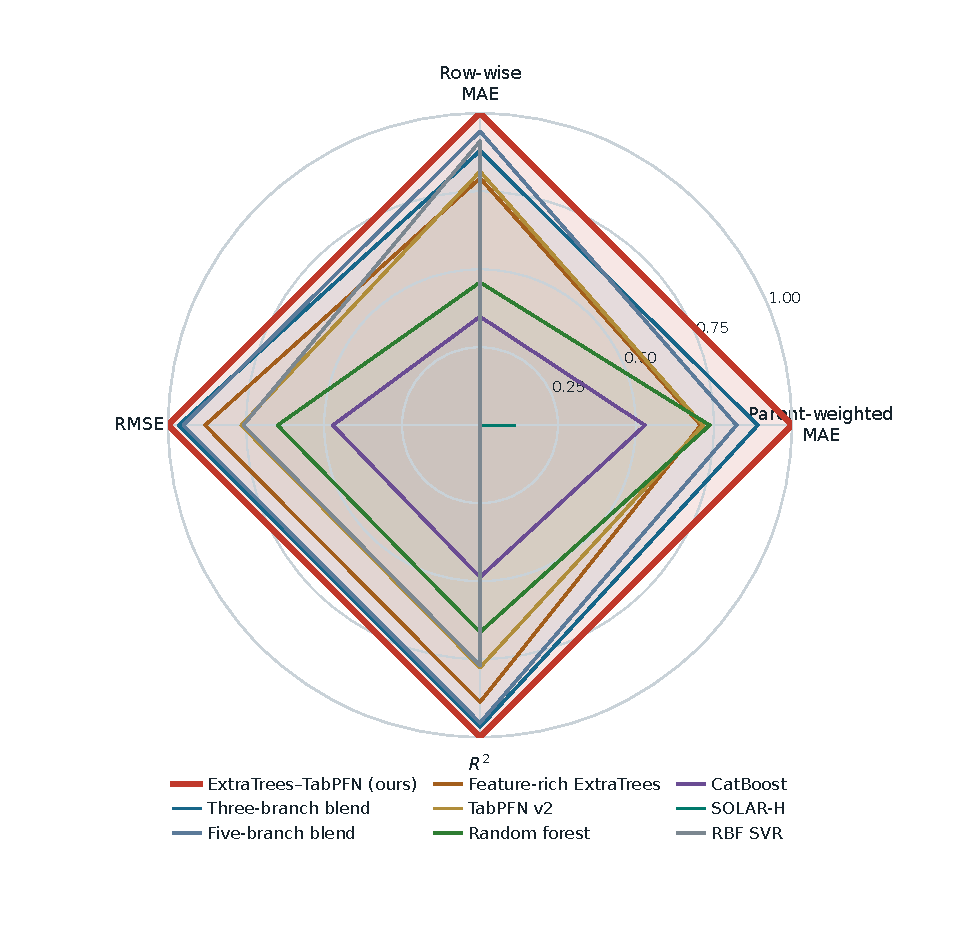
\includegraphics[width=0.78\linewidth]{model_radar.pdf}
\caption{Normalised radar comparison of the models across the four metrics (all axes are normalised to $[0,1]$ with a larger radius always better; the three error metrics are inverted).}
\label{fig:model_radar}
\end{figure}

\subsection{Ablation Analysis}

Figure~\ref{fig:v2_prediction_diagnostics}a shows the paired gains of the blend over its baselines together with the bootstrap intervals.

\begin{figure}[htbp]
\centering
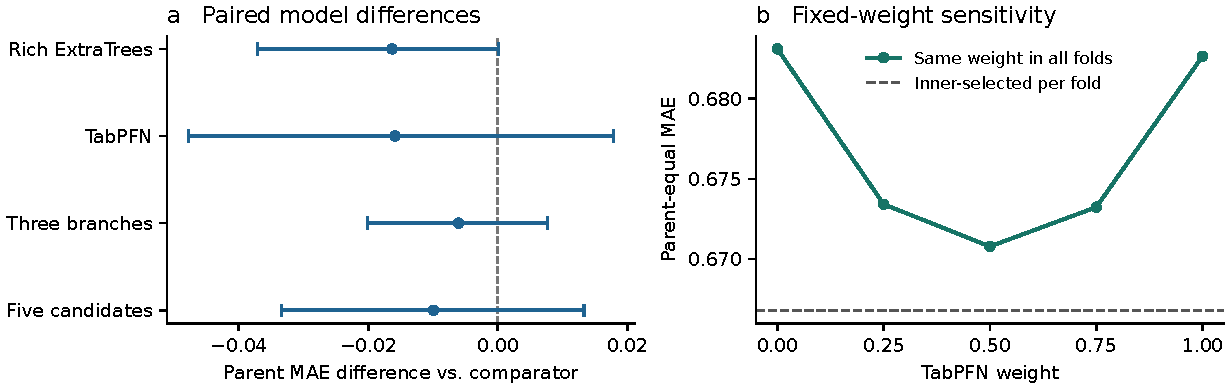
\includegraphics[width=\linewidth]{prediction_diagnostics.pdf}
\caption{Performance gains and weight sensitivity of the ExtraTrees--TabPFN blend. \textbf{a} paired differences in parent-weighted MAE against the baselines (negative means the blend is better; bars are 95\% bootstrap intervals). \textbf{b} parent MAE as a function of a fixed global weight $\alpha$ (the dashed line is the adaptive per-fold baseline).}
\label{fig:v2_prediction_diagnostics}
\end{figure}

Tracing the whole technical trajectory, three core refinements drive the gains: the leap from 23 base features to 869 explicit interaction features, which feeds polarity matching directly and narrows the error; the parent-equal sample weighting ($q=1$), which removes the head-parent bias and cuts the error by a further 0.023; and the context-attention TabPFN branch, which applies a local continuous correction and locks the parent MAE at the global optimum of 0.6668.

\subsection{Stratified Error Analysis}

At the parent level, the median per-parent MAE of SOLAR-H and the blend over the 128 unseen parents are 0.599 and 0.544. Across all 128 test parents, the blend beats SOLAR-H on 77 parents and beats the feature-rich ExtraTrees single model on 61.

To understand the behaviour across physicochemical environments, Table~\ref{tab:v2_target_band_errors} reports the two models' errors stratified by the measured log-solubility band.

\begin{table}[htbp]
\centering
\small
\setlength{\tabcolsep}{3.5pt}
\caption{Stratified errors of the two core models across measured-solubility bands (signed error is prediction minus measurement; positive means systematic overestimation, negative underestimation).}
\label{tab:v2_target_band_errors}
\begin{tabular}{lrrrrrr}
\toprule
& & & \multicolumn{2}{c}{SOLAR-H} & \multicolumn{2}{c}{ExtraTrees--TabPFN}\\
\cmidrule(lr){4-5}\cmidrule(lr){6-7}
Band & Records & Parents & Row-wise MAE & Signed error & Row-wise MAE & Signed error \\
\midrule
Extreme ($y \leqslant -4$) & 23 & 8 & 2.413 & $+2.396$ & 2.251 & $+2.250$ \\
Low ($-4 < y \leqslant -2$) & 321 & 56 & 0.997 & $+0.876$ & 0.874 & $+0.784$ \\
Moderate ($-2 < y \leqslant 0$) & 824 & 110 & \textbf{0.551} & $-0.184$ & \textbf{0.465} & $-0.120$ \\
High ($y > 0$) & 339 & 43 & 0.895 & $-0.873$ & 0.782 & $-0.772$ \\
\bottomrule
\end{tabular}
\end{table}

The stratified errors expose a chemically meaningful ``solubility cliff''.

In the moderate band ($-2 < y \le 0$), which holds 54.7\% of the samples, the blend performs exceptionally well---a row-wise MAE of just 0.465 and a signed bias of $-0.120$---delivering accurate continuous fits for routine pharmaceutical conditions.

In the extreme band ($y \le -4$, 23 records over 8 parents), both models' errors balloon (MAE above 2.2) and both systematically overestimate by more than $+2.2$ orders of magnitude. Take sucrose in chloroform at $25^\circ\text{C}$: the measured log-solubility is $-6.234$, but the model predicts $-2.536$ on average. The mechanism is thermodynamic: solubility depends not only on the liquid-phase solvation free energy (captured by 2D topological descriptors) but also, and more directly, on the lattice energy and solid-state packing of the pure crystal. Sucrose carries abundant hydroxyl groups that form a strong interlocking hydrogen-bond network in the solid, so desolvation and melting must overcome a large lattice-energy barrier, which is why it is so insoluble in chloroform. A pure 2D prediction, without an experimental melting point or three-dimensional unit-cell packing parameters, can only reason from liquid-phase polarity mismatch and therefore overestimates systematically. This is a practically important warning: for compounds predicted near the insoluble edge, solid-state polymorph and melting-point measurement should be scheduled first.

\subsection{Sensitivity and Randomness}

Across the outer five folds, the adaptively chosen TabPFN blend weights $\widehat\alpha$ are 0.25, 0.25, 0.0, 0.25, 0.50 (averaging about 0.25), and the ExtraTrees weighting exponent $q$ consistently prefers 1.

On weight robustness, Figure~\ref{fig:v2_prediction_diagnostics}b fixes the out-of-fold predictions and sweeps a constant global $\alpha$. Over $\alpha \in [0.25, 0.75]$ the parent-weighted MAE is 0.6734, 0.6708, 0.6732---a very flat basin that beats both single-branch endpoints (0.6831 at $\alpha=0$ and 0.6827 at $\alpha=1$). The blending gain is therefore tolerant of weight changes rather than depending on a brittle optimum.

On seed sensitivity, holding the same five-fold parent split and reporting seeds 17, 42, and 2026, the blend's parent-weighted MAEs are 0.6635, 0.6679, and 0.6690---a spread of only 0.0055. This low random variance confirms the stability of both the training strategy and the ensemble.

\subsection{Model Selection and Deployment}

Enlarging the candidate pool does not help. Adding CatBoost to form a three-branch ensemble gives a parent MAE of 0.6729; using all five candidate learners gives 0.6767. Both trail the two-branch ExtraTrees--TabPFN (0.6668).

Following Occam's razor, we therefore keep the two-branch blend as the final model. It holds the best generalisation and the lowest dispersion; relative to the three- or five-branch variants it avoids model bloat and storage overflow while simplifying the system, and under GPU acceleration it responds in under a second, which suits interactive real-time screening.
